\documentclass[12pt]{article}
\usepackage[utf8]{inputenc}
\usepackage[T1]{fontenc}
\usepackage[spanish]{babel}
\usepackage{graphicx}
\usepackage{geometry}
\usepackage{titlesec}
\usepackage{setspace}
\usepackage{hyperref}
\usepackage{enumitem}
\usepackage{listings}
\usepackage{xcolor}
\usepackage{framed}

% Configuración esencial para listings la vaina que permite mostrar código 
\definecolor{codebg}{rgb}{0.95,0.95,0.95}
\lstset{
    backgroundcolor=\color{codebg},
    basicstyle=\ttfamily\footnotesize,
    breaklines=true,
    frame=single,
    language=SQL,
    numbers=left,
    numberstyle=\tiny\color{gray},
    captionpos=b
}

% Configuración de página
\geometry{letterpaper, margin=2.5cm}
\setlength{\parskip}{1em}
\setlength{\parindent}{0pt}
\titleformat{\section}{\large\bfseries}{\thesection}{1em}{}
\titleformat{\subsection}{\normalsize\bfseries}{\thesubsection}{1em}{}

% Configuración de hipervínculos
\hypersetup{
    colorlinks=true,
    linkcolor=blue,
    urlcolor=blue,
    pdftitle={Tienda Online de Productos Electrónicos},
    pdfauthor={Aaron Rodrigo Ramos Reyes}
}

\begin{document}

% Portada
\begin{titlepage}
    \centering
    \vspace*{3cm}
    {\Huge\bfseries Sistemas Distribuidos \par}
    \vspace{2cm}
    {\Large Mini Plataforma de Video Streaming P2P con Microservicios\par}
    \vspace{3cm}
    {\large Autores:\par}
    \vspace{0.5cm}
    {\normalsize Aaron Rodrigo Ramos Reyes\par}
    {\normalsize Oscar Martinez Barrales\par}
    {\normalsize Oswaldo Mejia Garcia\par}
    \vfill
    {\large Universidad Autonoma Metropolitana\par}
    {\large Fecha: \today\par}
\end{titlepage}

% Índice
\tableofcontents
\newpage

% Sección de introducción
\section{Introducción}  

El presente proyecto consiste en la implementación de una \textbf{mini plataforma de video streaming P2P con microservicios}, cuyo objetivo es permitir que diferentes nodos intercambien fragmentos de video de manera distribuida, sin depender de un único servidor central para el envío de datos.

\subsection*{Planteamiento del Problema}
Las plataformas de streaming tradicionales dependen de un servidor central que entrega el contenido directamente a cada usuario. Esto genera un cuello de botella cuando muchos usuarios solicitan el mismo video.  
En este proyecto se busca aprovechar el \textbf{modelo P2P} para que cada nodo no solo consuma, sino que también comparta fragmentos con otros, reduciendo la carga central.

\subsection*{Estructura de la Solución}
La solución se basa en tres elementos clave:
\begin{enumerate}
    \item \textbf{Servicio Central (Registry Service)}: Registra nodos y mantiene un mapeo de qué fragmentos posee cada uno.
    \item \textbf{Nodos P2P}: Almacenan y comparten fragmentos de video, comunicándose directamente para transferir datos.
    \item \textbf{Sistema Pub/Sub con Redis}: Notifica a los nodos cuando hay nuevos fragmentos disponibles.
\end{enumerate}

\subsection*{Diagrama de Arquitectura}
Diseño del esquema general del sistema, incluyendo el servicio central, los nodos P2P y el canal de comunicación Pub/Sub.

\begin{center}
    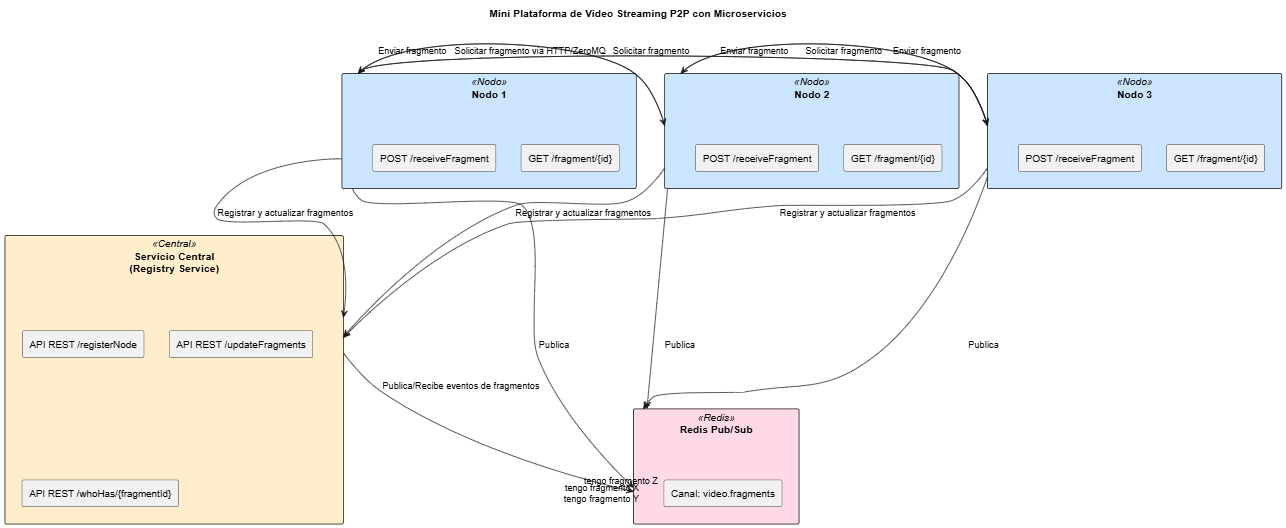
\includegraphics[width=\textwidth]{Diagramas/Diagrama.png}
\end{center}







\end{document}